\section{Gaussian Processes}
\label{gp}

Given an exosuit parameterization space $\mathbb{X} \subset \mathbb{R}^m$ and an unknown, noisy energetic cost function $f$ that is expensive to evaluate, we aim to find the solution to the minimization problem
\begin{align}
  x^* = \argmin_{x \in \mathbb{X}} f(x),
\end{align}
by iteratively choosing points to evaluate until a finite time constraint is met. Bayesian Optimization, our sequential design strategy, computes a posterior distribution on possible objective functions given all previous evaluations and optimizes an acquisition function on this distribution to globally select the next value of $x$ to evaluate, typically in a way that carefully balances exploration and exploitation. The distribution over $f$ is modeled as a Gaussian process \citep{Rasmussen2006}, $\mathbb{G}$, 
\begin{align}
  f \sim \mathbb{G}(\mu, \kappa), 
\end{align}
where $\mu : \mathbb{X} \rightarrow \mathbb{R}$ is a mean function typically set to zero, and $\kappa : \mathbb{X}\times \mathbb{X} \rightarrow \mathbb{R}$ is a covariance kernel that characterizes the correlation between different points in the domain. The most common example is the squared exponential kernel
\begin{align}
  \kappa(x_i, x_j \vert \theta) = \sigma_\theta^2 \exp(-\frac{1}{2}d^2(\frac{x_i}{l}, \frac{x_j}{l}))
\end{align}
with parameters $\theta = [\sigma_\theta^2, l]$ where $l$ is either a scalar or vector of dimension $m$. The Matérn kernel is a more generalized form of the squared exponential, defined as
\begin{align}
	\kappa(x_i, x_j \vert \theta) = \sigma_\theta^2\frac{2^{1-\nu}}{\Gamma(\nu)}(\sqrt{2\nu} d(\frac{x_i}{l}, \frac{x_j}{l}))^\nu K_\nu (\sqrt{2\nu} d(\frac{x_i}{l}, \frac{x_j}{l}))
\end{align}
with an additional parameter $\nu$ and $K_\nu$ is a modified Bessel function. 
\section{GP Regression and Acquisition Functions}
\label{gp_acq}
By definition of a GP, any collection of points forms a multivariate normal distribution defined by $\mu$ and $\kappa$. More formally, given some training samples $\mathbb{S} = \{(x_i, y_i)\}_{i=1}^n$ and assuming a Gaussian noise model $y_i \sim f(x_i) + \mathcal{N}(0, \sigma_n^2)$, the posterior distribution at $x$ is a normal with mean $\bar{\mu}(x)$ and variance $\bar{\sigma}^2(x)$ evaluated as
\begin{gather}
  \bar{\mu}(x) = K(X, x)^T[K(X, X) + \sigma_n^2 I]^{-1}Y \\
  \bar{\sigma}^2(x) = \kappa(x, x\vert \theta) - K(X, x)^T[K(X,X) + \sigma_n^2 I]^{-1}K(X,x) \\
  K(X,x)_i = \kappa(x_i, x\vert \theta) \nonumber\\
  K(X,X)_{ij} = \kappa(x_i, x_j\vert \theta) \nonumber,
\end{gather}
where $X = \{x_i\}_{i=1}^n$ and $Y = \{y_i\}_{i=1}^n$. 
\begin{figure}[t]
\centering
\includegraphics[width=\textwidth]{gp_regression.png}
\caption{Sample GP Regression of a function using squared exponential and Matérn kernels.}
\label{fig:gp_regression}
\end{figure}

Given a distribution at point $x$, an acquisition function captures how attractive that point is to sample next. A common choice of acquisition function is Expected Improvement (EI), which returns the expected reduction in cost over the best parameters observed so far. For the given GP model, EI can be computed in closed form: 
\begin{align}
  EI(x\vert \mathbb{S}) &= z\bar{\sigma}(x)\Phi(z) + \bar{\sigma}(x)\phi(z) \\
  z &= \frac{\min(Y) - \bar{\mu}(x) + \xi}{\bar{\sigma}(x)}\nonumber,
\end{align}
where $\xi$ is a scaling parameter to adjust the tradeoff between exploration-exploitation \citep{Lizotte:2008:PBO:1626686}. Using EI, the next point is chosen as $x^* = \argmax_{x} EI(x \vert \mathbb{S})$. Figure \ref{fig:ei} shows a few iterations of Bayesian Optimization on a sample function.

\section{Hyperparameter Optimization and Student-t Noise Model}
\label{gp_hyperparam}
The values of the hyperparameters in the kernel function are critical to determining the posterior distribution. Typically, these hyperparameters are tuned to sampled points with a maximum a posteriori (MAP) point estimate \citep{NIPS2012_4522,GPstuff}. Specifically, assuming our Gaussian noise model we have an analytical solution

\begin{gather}
\argmax_{\theta, \sigma_n^2} \text{ } log P(\mathbb{S}\vert \theta, \sigma_n^2) + log P(\theta, \sigma_n^2)\\
=log \int p(Y\vert f, \sigma_n^2)p(f\vert X,\theta)df + log P(\theta, \sigma_n^2)\nonumber\\
= -\frac{n}{2}log(2\pi) - \frac{1}{2}log(K(X,X) + \sigma_n^2 I) - \frac{1}{2}Y^T(K(X,X) + \sigma_n^2 I)^{-1}Y + log P(\theta, \sigma_n^2)\nonumber
\end{gather}


\begin{algorithm}[t]
\caption{Bayesian Optimization Outline}
\label{alg:bayesopt}
\begin{algorithmic}
\State \textkeyword{Objective Function} $F(x)$
\State \textkeyword{Acquisition Function} $g(\mu, \sigma^2)$
\State \textkeyword{Specify Exploration Points } $\mathbb{E} = \{e_1, e_2, ..., e_n\}$
\State \textkeyword{Training Samples } $\mathbb{S}$
\For{i=1}{n}
  \State $\mathbb{S} = \mathbb{S} \cup \{e_i, F(e_i)\}$
\End
\While{t < T}
  \State Update GP Hyperparameters $\theta, \sigma_n^2$
  \State Given $f(x\vert \theta, \sigma_n^2, \mathbb{S}) \sim \mathcal{N}(\mu_x, \sigma_x^2)$,
  \State $x^* = \argmax_{x \in \mathbb{X}} g(\mu_x, \sigma_x^2)$
  \State $\mathbb{S} = \mathbb{S} \cup \{x^*, f(x^*)\}$
\End
\end{algorithmic}
\end{algorithm}


Instead of using a single point estimate, a full Bayesian approach would involve marginalizing out the hyperparameters through an MCMC approximation. This would be particularly beneficial in the case that the posterior is multi-modal or sensitive to small changes in parameter values. Many sampling approaches have been proposed, and we refer the reader to \cite[Chapter~14]{barber2011bayesian} for a summary. 

The MCMC approach is also used in more complex noise models whose posterior distribution and marginal likelihood are no longer analytically tractable. \citet{NIPS2009_3806,Jylanki:2011:RGP:1953048.2078209} developed a more robust noise model based on the Student-t distribution to handle occurrences of large outliers in the collected data. The noise model follows

\begin{align}
p(y\vert f,\sigma_n^2,\nu) = \frac{\Gamma (\frac{\nu + 1}{2})}{\Gamma(\frac{\nu}{2})\sqrt{\nu\pi}\sigma_n})(1 + \frac{(y-f)^2}{\nu\sigma_n^2})^{\frac{-(\nu + 1)}{2}}
\end{align} 
where $\nu$ is the degrees of freedom. A Gibbs sampler can be performed through a hierarchical model
\begin{align}
\begin{split}
y\vert f &\sim \mathcal{N}(f, V)\\
V &\sim \text{Inv-}\chi^2(\nu, \sigma_n^2),
\end{split}
\end{align}
with $\theta$ alternately sampled according to the Gaussian Process. Figure \ref{fig:mcmcvsmap} shows a comparison of the robust Student-t noise with the standard Gaussian noise.

\begin{figure}[t]
\centering
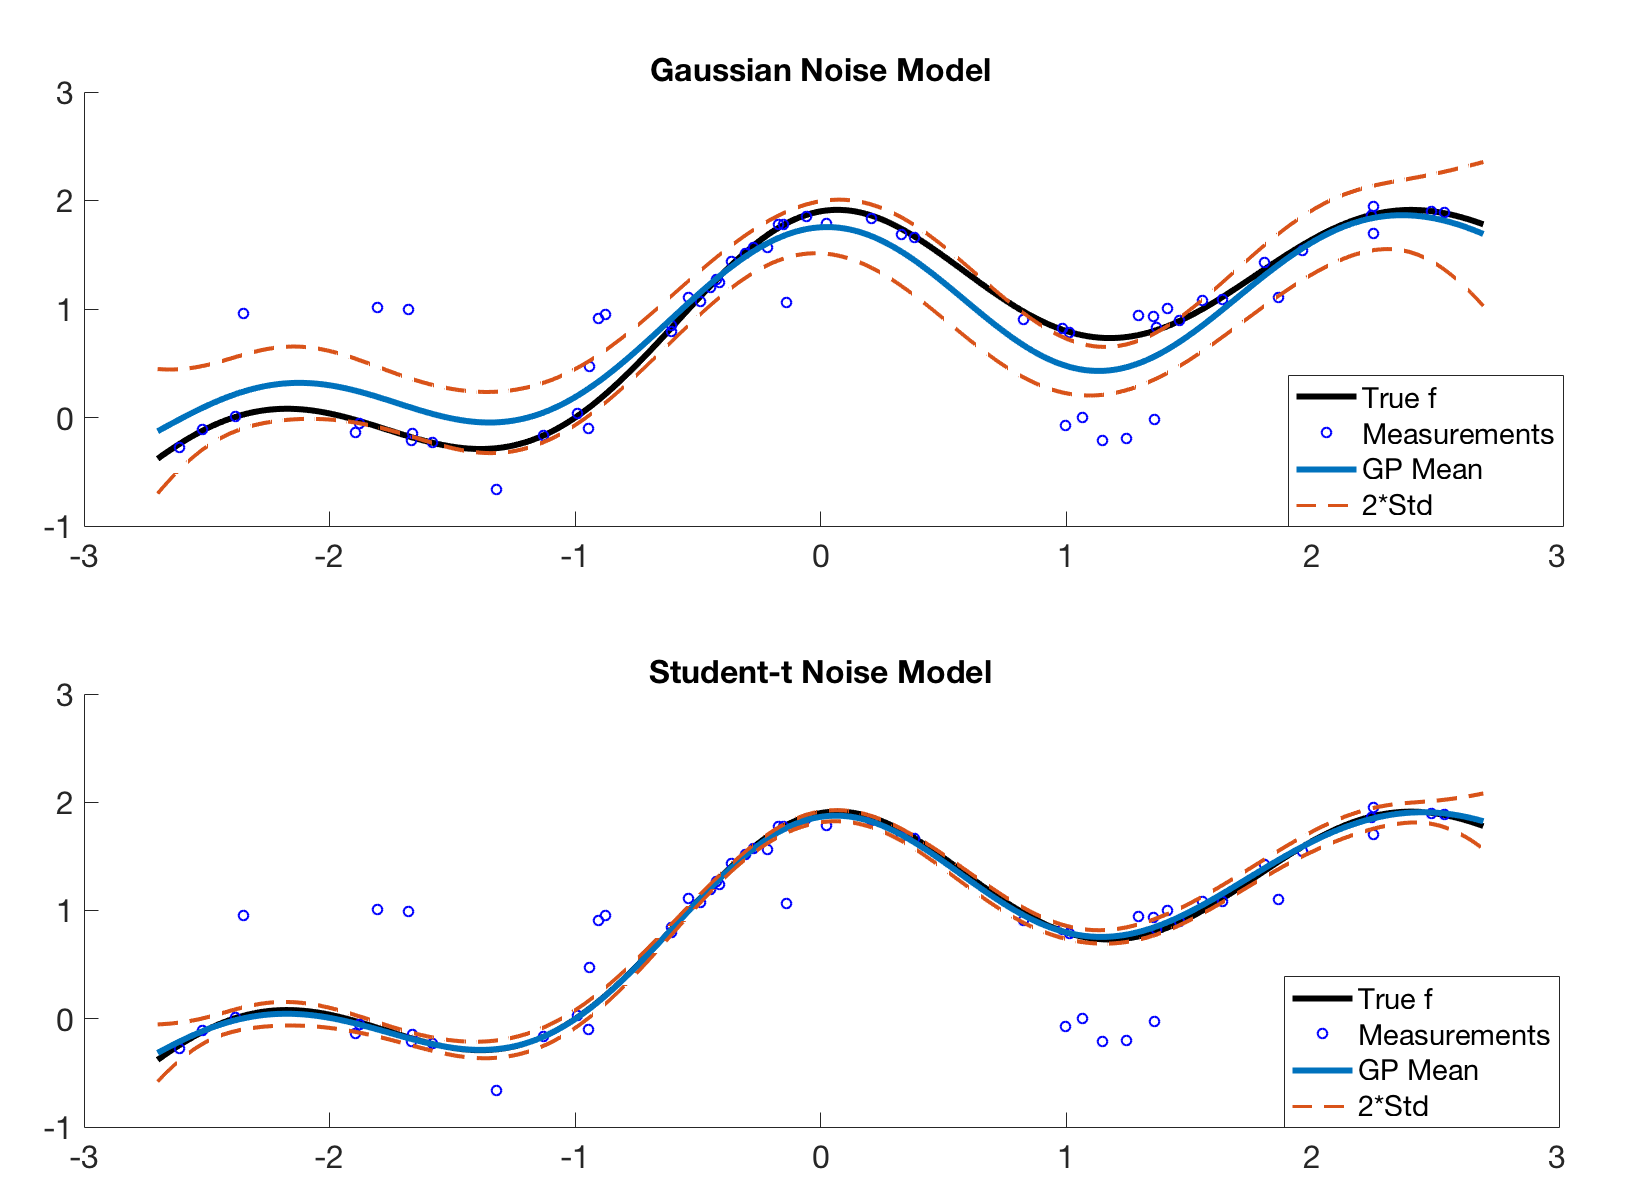
\includegraphics[width=\textwidth]{mcmcvsmap}
\caption{Gaussian MAP estimate vs. Student-t Gibbs Sampler. Data points added with Gaussian noise including some outliers with very high variance.}
\label{fig:mcmcvsmap}
\end{figure}
